\frame{
  \frametitle{Lógica Nebulosa}
  \begin{block}{}
    \begin{figure}
      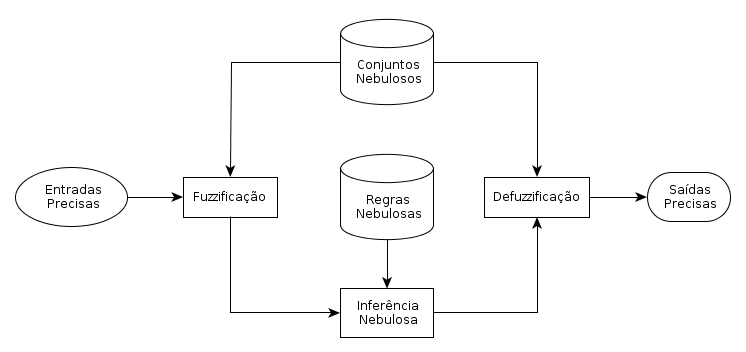
\includegraphics[width=0.8 \linewidth]
      {imgs/arquitetura_fuzzy}
      \caption{Arquitetura Funcional Genérica de um Sistema
      Nebuloso}
    \end{figure}
  \end{block}
}

\frame{
  \frametitle{Lógica Nebulosa}
  \begin{block}{}
    \textbf{Exemplo} Determinar o valor da apólice de seguro
    a ser paga pelo cliente João, cuja idade é 35 anos e a
    pressão arterial é de (130,75). As regras são:
    \begin{itemize}
      \item \emph{SE} idade é \textit{meia-idade} \emph{E}
            pressão arterial é \textit{baixa} \emph{ENTÃO}
            seguro é \textit{baixo}
      \item \emph{SE} é \textit{jovem} \emph{E} pressão
            arterial é \textit{alta} \emph{ENTÃO} seguro
            é \textit{alto}
    \end{itemize}
  \end{block}
}

\frame{
  \frametitle{Lógica Nebulosa}
  \begin{block}{}
    Se $\mu_{meia-idade}(35)= 0.8, \mu_{jovem}(35)= 0.6,
    \mu_{Alta}(130,70)=0.5$ e $\mu_{Baixa}=0.6$, tem-se:
    \begin{itemize}
      \item $0.8$ \emph{E} $0.6$ = $Min \lbrace 0.8,
      0.6\rbrace = 0.6 = \mu_{seguro-baixo}(X_1)$
      \item $0.6$ \emph{E} $0.5$ = $Min \lbrace 0.6,
      0.5\rbrace = 0.5 = \mu_{seguro-alto}(X_2)$
    \end{itemize}
  \end{block}
  \begin{block}{}
    Aplicando o processo de defuzzificação, obtem-se:
    \begin{itemize}
      \item $X_1 = 700$ e $X_2 = 800$
    \end{itemize}
	Assim, o valor final da apólice de seguro seria:
	\[
	Seguro = \frac{(0.6 \times 700)+(0.5 \times 800)}
	{0.6+0.5} = 745.45 reais 
	\]    
  \end{block}    
}

\frame{
  \frametitle{Lógica Nebulosa}
  \begin{block}{}
    \begin{figure}
      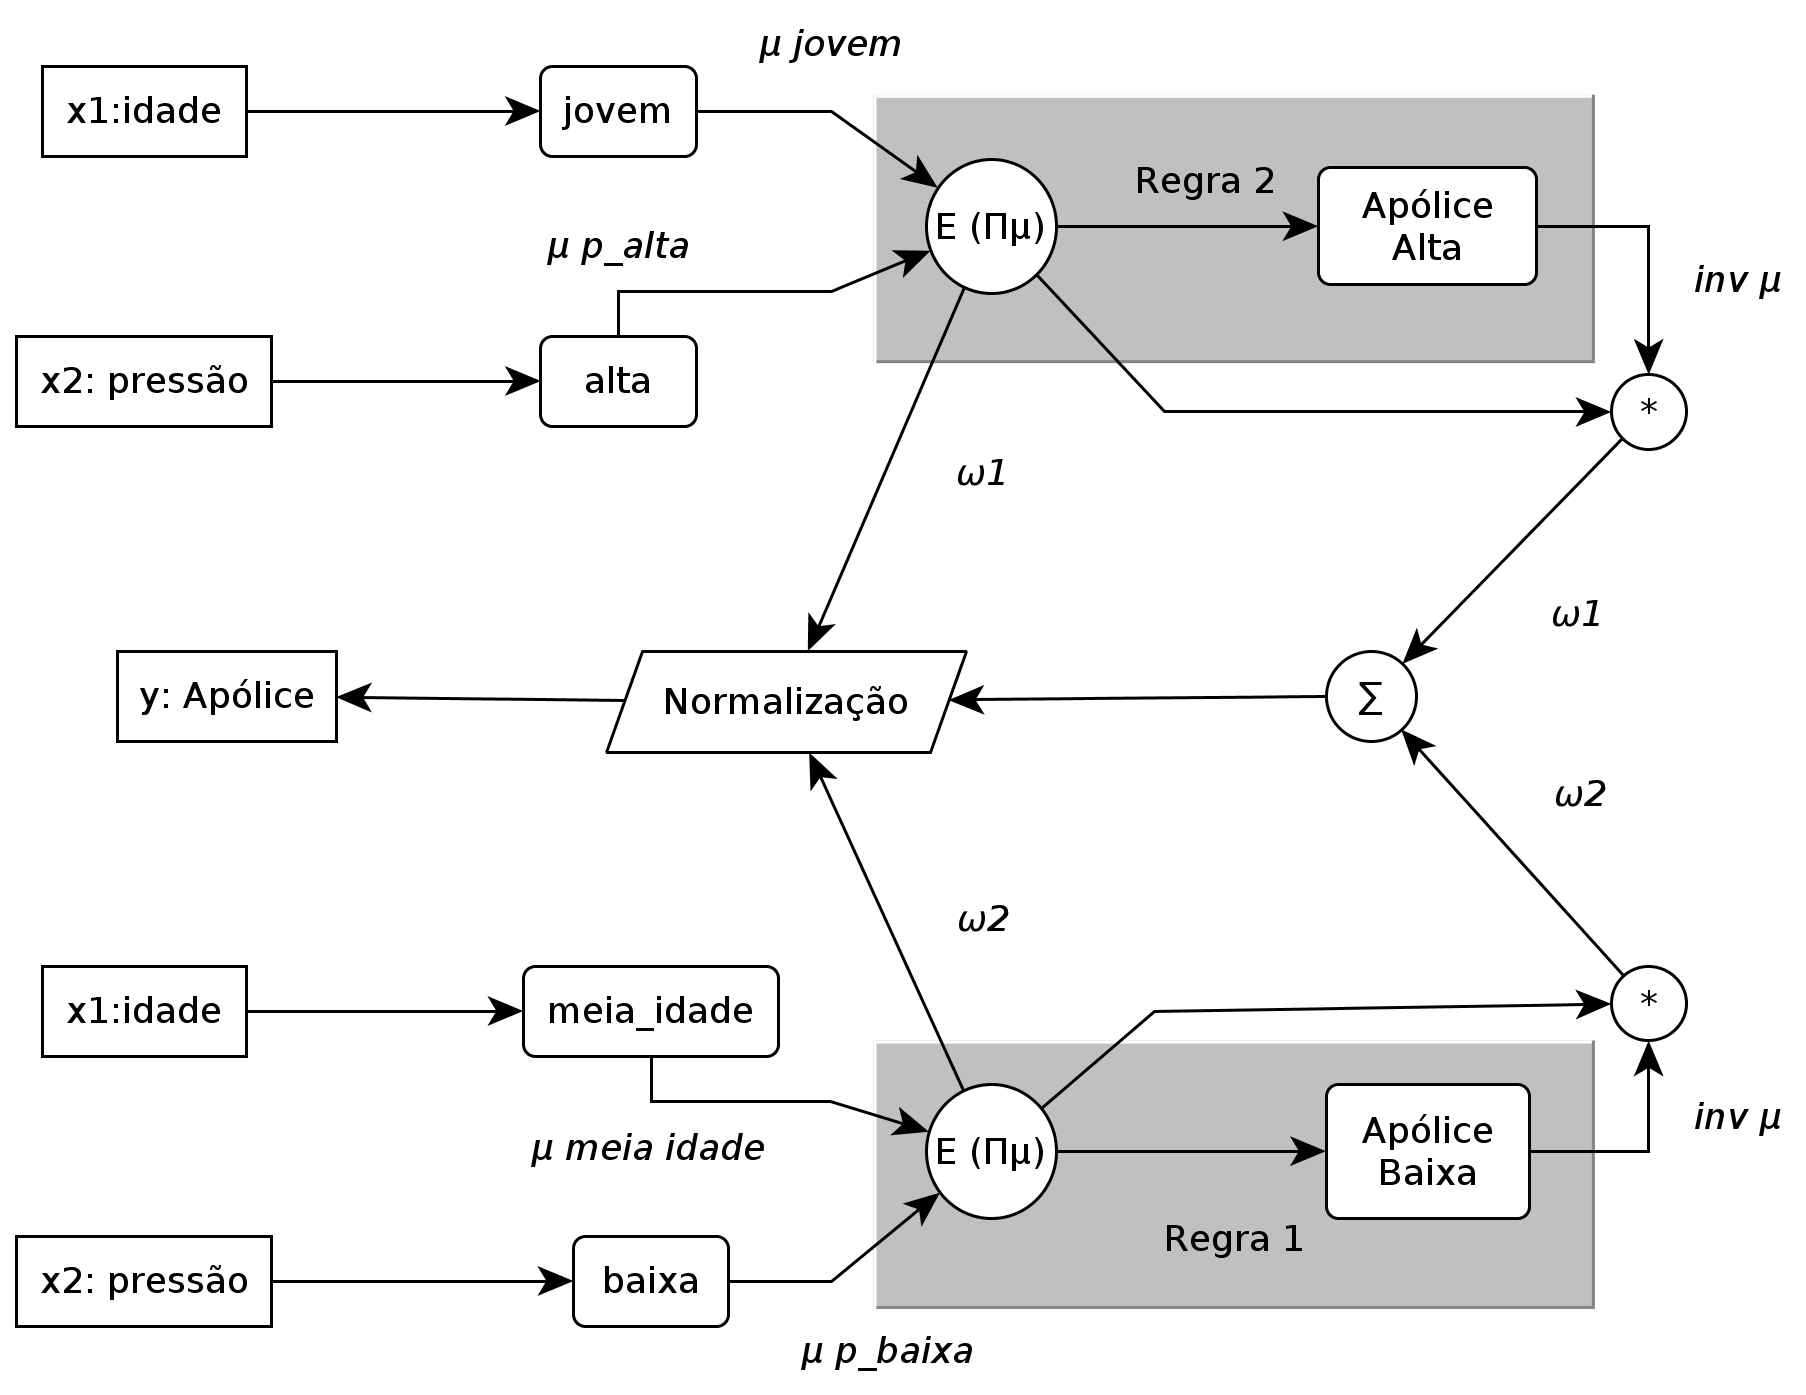
\includegraphics[width =0.6 \linewidth]
      {imgs/ex_logica_fuzzy}
      \caption{Exemplo de Aplicação}
    \end{figure}
  \end{block}
}

\frame{
  \frametitle{Lógica Nebulosa (SAM)}
  \begin{block}{}
    $$
    F(x) = \frac{\sum w_i.a_i(x).V_i.c_i}{\sum w_j.a_j(x).V_j}
    $$

    Com o volume/área $V_j$ e o centroide $c_j$ são dados por:

    $$
    V_j = \int{b_j(y_1, \cdots ,y_p)}_{\Re^{p}}.dy_1
    \cdots dy_p > 0
    $$

    $$
    c_j = \frac{\int{y.b_j(y_1,\cdots,y_p)}_{\Re^{p}}
    .dy_1 \cdots dy_p}{V_j}
    $$
  \end{block}
}